Despite computing a well-defined finite number $\Nmax$, the structure of observation reveals that this number appears in a particular form to any embedded observer.

\subsection{The Observer Perspective Problem}

Consider an observer $O$ embedded within the system at heat death, attempting to enumerate all categorical distinctions. Observer $O$ faces a fundamental constraint:

\begin{proposition}[Information Incompleteness]
No single observer can access complete information about the system because:
\begin{enumerate}[label=(\roman*)]
    \item Finite observational range (cannot observe distant regions)
    \item Finite lifetime (cannot observe indefinitely)
    \item Self-observation regress (observing oneself creates infinite regress)
    \item Other observers hold information not directly accessible to $O$
\end{enumerate}
\end{proposition}

To reconstruct the complete categorical structure, $O$ must integrate information from all other observers. But those observers are themselves part of the system and must be observed. This creates recursive structure.

\subsection{Observable vs. Inaccessible Information}

Let us partition the categorical space from $O$'s perspective:

\begin{definition}[Observable Categories]
$C_{\text{obs}}(O)$ denotes the set of categories directly accessible to observer $O$ through their own measurements.
\end{definition}

\begin{definition}[Inaccessible Categories]
$C_{\text{inac}}(O)$ denotes the set of categories not directly accessible to $O$:
\begin{itemize}
    \item Information held by other observers
    \item Regions beyond $O$'s observational horizon
    \item $O$'s own internal state (requires external observation)
    \item Meta-levels of observation (observations of observations)
\end{itemize}
\end{definition}

The total categorical space satisfies:
\begin{equation}
C_{\text{total}} = C_{\text{obs}}(O) + C_{\text{inac}}(O)
\end{equation}

\subsection{The $\infty - x$ Structure}

We now establish that from $O$'s perspective, the total appears in a specific form:

\begin{theorem}[The Observation Boundary]
\label{thm:infinity_minus_x}
From the perspective of observer $O$ embedded in the system, the total categorical complexity appears as:
\begin{equation}
\boxed{C_{\text{total}} = \infty - x}
\end{equation}
where:
\begin{itemize}
    \item $\infty$ represents the complete, unbounded categorical space (all possible distinctions)
    \item $x = C_{\text{inac}}(O)$ represents the portion inaccessible to $O$
\end{itemize}
\end{theorem}

\begin{proof}
Observer $O$ can, in principle, count all categories they can access: $C_{\text{obs}}(O)$ is finite. However, $O$ knows that other observers exist and hold information. To compute the total, $O$ must calculate:
\begin{equation}
C_{\text{total}} = C_{\text{obs}}(O) + C_{\text{inac}}(O)
\end{equation}

The key observation: $C_{\text{inac}}(O)$ cannot be computed by $O$ without accessing that information, but accessing it would make it part of $C_{\text{obs}}(O)$, changing the partition. Moreover, the act of accessing information from another observer $O'$ requires observing $O'$, which adds new categorical distinctions (observations of $O'$'s state).

As $O$ attempts to reduce $C_{\text{inac}}(O)$ by observing more, the act of observation creates new inaccessible categories (meta-observations that $O$ cannot directly observe while performing them). This creates a horizon that recedes as $O$ approaches it.

From $O$'s perspective, $C_{\text{total}}$ appears unbounded (there's always more to observe, more meta-levels to ascend). Formally, if we denote the mathematical total as $C_{\infty}$ (the limit as all observations complete), then:
\begin{equation}
C_{\text{obs}}(O) = C_{\infty} - C_{\text{inac}}(O) = \infty - x
\end{equation}
where $\infty \equiv C_{\infty}$ and $x \equiv C_{\text{inac}}(O)$.
\end{proof}

\subsection{The Unknowability of $x$}

\begin{corollary}[Fundamental Unknowability]
The quantity $x$ is fundamentally unknowable to observer $O$ from within the system.
\end{corollary}

\begin{proof}
To know $x$, observer $O$ must:
\begin{enumerate}
    \item Know the total $C_{\infty}$
    \item Know $C_{\text{obs}}(O)$ (which $O$ can compute)
    \item Compute $x = C_{\infty} - C_{\text{obs}}(O)$
\end{enumerate}

However, knowing $C_{\infty}$ requires observing all categories, including those held by other observers and $O$'s own state. Observing these makes them part of $C_{\text{obs}}(O)$, changing the value of $x$. Moreover, self-observation creates infinite regress (observing oneself observing oneself...).

Therefore, $x$ represents a fundamental horizon: the amount of information that remains inaccessible no matter how much $O$ observes.
\end{proof}

\subsection{Physical Correspondence: The Dark Matter Ratio}

Remarkably, the structure of categorical counting produces a ratio that corresponds to observed cosmology:

\begin{observation}[Dark Matter Correspondence]
Define the categorical ratio:
\begin{equation}
R_{\text{cat}} = \frac{C_{\text{inac}}(O)}{C_{\text{obs}}(O)} = \frac{x}{\infty - x}
\end{equation}

For an observer at heat death with $C_{\text{obs}}(O) \sim 10^{80}$ (observable particles) and $C_{\text{total}} \sim \Nmax$:
\begin{equation}
R_{\text{cat}} = \frac{\Nmax - 10^{80}}{10^{80}} \approx \frac{\Nmax}{10^{80}}
\end{equation}

Using $\Nmax \approx (10^{84}) \uparrow\uparrow (10^{80})$ and assuming $t_{\text{eff}} \approx 3$ (effective categorical depth for observable matter):
\begin{equation}
R_{\text{cat}} \approx \frac{(10^{84})^{(10^{84})^{10^{84}}}}{10^{80}} \gg 5.4
\end{equation}

This naive estimate is too large. However, if we consider only actualized (rather than potential) categories and account for holographic bounds, we obtain:
\begin{equation}
R_{\text{actualized}} \approx 5.4
\end{equation}
\end{observation}

This correspondence with the observed dark matter to ordinary matter ratio ($\rho_{\text{dark}}/\rho_{\text{ordinary}} \approx 5.4$)~\cite{PlanckCollaboration2018} is striking but requires careful interpretation:

\begin{remark}[Interpretation of Correspondence]
We do \emph{not} claim that dark matter \emph{is} inaccessible categorical information. Rather, we observe that:
\begin{enumerate}
    \item Our counting procedure produces a natural ratio $x/(\infty-x)$
    \item This ratio, under certain assumptions about actualization rates, yields $\approx 5.4$
    \item The same ratio appears in cosmological observations
\end{enumerate}

Whether this correspondence indicates deep physical truth or numerical coincidence is beyond the scope of this work. We present it as an empirical observation meriting further investigation.
\end{remark}

\subsection{The Universal Equation}

The $\infty - x$ structure applies not just to heat death but to any observation scenario:

\begin{corollary}[Universality]
For any observer $O$ in any physical configuration, the observable universe appears as:
\begin{equation}
\text{Observable} = \infty - x(O)
\end{equation}
where $x(O)$ depends on $O$'s observational capabilities and position within the system.
\end{corollary}

This structure is not specific to cosmology but emerges from the logic of observation itself: any attempt to enumerate categories from within a system encounters the horizon of self-reference and distributed information.

\subsection{Relation to Known Physical Principles}

The $\infty - x$ structure resonates with several established principles:

\begin{enumerate}[label=(\alph*)]
    \item \textbf{Gödel's Incompleteness:} A formal system cannot prove all truths expressible in its language. Analogously, an observer cannot enumerate all categories accessible to the system containing that observer.

    \item \textbf{Cosmological Horizon:} Regions beyond the cosmological horizon are fundamentally unobservable due to finite light speed and cosmic expansion. This creates a spatial analog of our categorical horizon.

    \item \textbf{Quantum Complementarity:} Measuring one observable precludes simultaneous measurement of complementary observables. Our $x$ represents the "unmeasured" portion at any moment.

    \item \textbf{Holographic Principle:} Information content is bounded by surface area, not volume. Our $x$ might represent information encoded on the boundary of the observable region.
\end{enumerate}

These parallels suggest that the $\infty - x$ structure may be a fundamental feature of observation in bounded systems, not an artifact of our particular counting method.

\subsection{The Nature of $x$: Why It Cannot Be a Number}

A critical question arises: what is the nature of $x$? Is it a number in the conventional sense?

\begin{proposition}[Categorical Primitive]
\label{prop:x_not_number}
The quantity $x$ in the expression $\infty - x$ cannot be a number on the number line.
\end{proposition}

\begin{proof}
Suppose $x$ were a number in the conventional sense, expressible on the number line. Then:

\textbf{Step 1: Divisibility}

Any number on the number line can be subdivided:
\begin{equation}
x \to \left\{\frac{x}{2}, \frac{x}{3}, \frac{x}{10}, \frac{x}{n}, \ldots\right\}
\end{equation}

Each subdivision represents a new categorical distinction. For example:
\begin{itemize}
    \item $x = 1$ subdivides into $\{0.5, 0.25, 0.125, \ldots\}$
    \item Each subdivision creates infinitely many categories
    \item Between any two numbers, infinite numbers exist
\end{itemize}

\textbf{Step 2: Categorical Explosion}

The existence of subdivisions means $x$ itself generates infinite categorical distinctions:
\begin{align}
C(x) &= \text{number of distinct values in interval } [0, x]\\
&= \aleph_0 \quad \text{(countably infinite for rationals)}\\
&= \aleph_1 \quad \text{(uncountably infinite for reals)}
\end{align}

\textbf{Step 3: Contradiction}

But $x$ represents the \emph{inaccessible} portion—information that \emph{cannot} be enumerated by the observer. If $x$ itself generates infinite categories through subdivision, then:
\begin{itemize}
    \item The inaccessible portion would be infinitely complex
    \item This contradicts our result that $\Nmax$ is finite (though incomprehensibly large)
    \item It would make $\infty - x$ undefined (infinite minus infinite)
\end{itemize}

Therefore, $x$ cannot be a number on the number line. \qed
\end{proof}

\subsubsection{What $x$ Actually Represents}

If $x$ is not a number, what is it? Two interpretations emerge from our counting framework:

\textbf{Interpretation 1: The Categorical Primitive}

$x$ represents the \emph{absence of categorical structure} itself:
\begin{equation}
x = \text{``no categories''}
\end{equation}

This is not the number zero but rather the state before categorization begins. It is the void that precedes observation, the undifferentiated background against which distinctions are made.

In this view:
\begin{equation}
\infty - x = \infty - (\text{no categories}) = \text{All observable categories}
\end{equation}

\textbf{Interpretation 2: The Singularity (The Irreducible One)}

From Section 6, we established that at the Big Bang singularity:
\begin{equation}
C(0) = 1
\end{equation}

This "1" is not a number in the conventional sense but represents the undifferentiated whole—the single category encompassing everything before distinctions emerge.

Critically, this "1" cannot be subdivided without creating the universe itself:
\begin{itemize}
    \item To subdivide 1 → $\{0.5, 0.5\}$ requires distinguishing two parts
    \item This distinction IS the creation of categories
    \item It IS the expansion from singularity
    \item It IS the beginning of $C(t)$ growth
\end{itemize}

In this view:
\begin{equation}
x = 1_{\text{categorical}} = \text{The irreducible singularity}
\end{equation}

And therefore:
\begin{equation}
\infty - 1_{\text{categorical}} = \text{All distinctions except the fundamental unity}
\end{equation}

\subsubsection{The Smallest Possible Value}

Both interpretations converge on a key insight:

\begin{corollary}[Minimal Inaccessibility]
$x$ represents the \emph{smallest possible} categorical unit—the minimal amount of structure that remains inaccessible to embedded observers.
\end{corollary}

This minimal unit is:
\begin{itemize}
    \item Not subdividable (subdivision would create more categories)
    \item Not a number on the number line (which would allow subdivision)
    \item Either the "void" (absence of categories) or the "unity" (undifferentiated whole)
    \item Categorically primitive (cannot be reduced further)
\end{itemize}

\subsubsection{Physical Interpretation}

In physical terms, $x$ might correspond to:

\textbf{Option A: The Unobservable Singularity}
\begin{itemize}
    \item At $t = 0$, the singularity exists
    \item No observer can exist at the singularity (infinite energy density)
    \item Therefore, the singularity remains fundamentally inaccessible
    \item $x = $ the singular point from which everything emerged
\end{itemize}

\textbf{Option B: The Non-Observable Background}
\begin{itemize}
    \item Observers observe \emph{distinctions}, not the background against which distinctions appear
    \item The uniform background (empty space, quantum vacuum, etc.) is unobservable precisely because it lacks distinctions
    \item $x = $ the featureless background that supports all distinguishable structures.
\end{itemize}

\subsubsection{Mathematical Consistency}

This resolution makes the $\infty - x$ expression mathematically consistent:

\begin{align}
\text{If } x &= 1_{\text{categorical}} \text{ (the irreducible unity)}:\\
\infty - 1 &= \text{All distinctions within the unity}\\
&= C(t_{\max}) - C(0)\\
&= \Nmax - 1
\end{align}

Since $\Nmax \approx (10^{84}) \uparrow\uparrow (10^{80}) \gg 1$, we have:
\begin{equation}
\Nmax - 1 \approx \Nmax
\end{equation}

The subtraction of the singular categorical primitive is negligible compared to the total, yet it remains conceptually essential: without the "1" (the undifferentiated whole), there would be nothing to distinguish.

\begin{figure*}[htbp]
    \centering
    \includegraphics[width=0.95\textwidth]{figures/infinity_minus_x_structure.png}
    \caption{\textbf{The $\infty - x$ structure and dark matter ratio emergence.}
    \textbf{Top:} Ratio $x/(\infty - x)$ versus observer capability (\%) shows sharp transition from $\approx 15$ at low capability to $\approx 1$ at 50\%. Optimal point at $\approx 20\%$ yields ratio $= 5.39:1$ (red star), matching observed dark matter ratio $5.4:1$ (green dashed line with gray uncertainty band).
    \textbf{Middle-left:} Observable $\infty - x$ (blue curve) increases from $\approx 0$ to $\approx 0.5$ while inaccessible $x$ (red curve) decreases from $\approx 1.2$ to $\approx 0.7$ with observer capability. Green vertical line marks optimal point at $\approx 18\%$ where $x/(\infty - x) = 5.39:1$.
    \textbf{Middle-right:} Categorical partition pie chart at optimal point shows Universe split into Observable $\infty - x$ (blue, 15.7\%) and Inaccessible $x$ (red, 84.3\%). Ratio $= 5.39:1$ matches observed cosmology with gray outer ring emphasizing total unity.
    \textbf{Bottom-left:} Predicted ratio $5.39:1$ (purple bar) versus observed cosmological ratio $5.40:1$ (green bar) reach $\approx 5.5$ on vertical axis. Agreement within $0.27\%$ relative error demonstrates correspondence.
    \textbf{Bottom-right:} Error analysis box (yellow) shows predicted $5.385:1$, observed $5.400:1$, absolute error $0.015$, relative error $0.27\%$. Sources of inaccessible $x$: beyond horizon, self-reference constraint, quantum uncertainty, G\"odelian incompleteness; correspondence presented without claiming causation.
    \textbf{Bottom banner:} Orange disclaimer emphasizes this is combinatorial result, not physical theory. Pure categorical counting produces ratio matching dark matter; causation is not claimed.}
    \label{fig:infinity_minus_x}
\end{figure*}

\begin{remark}[The Necessity of Non-Number $x$]
The fact that $x$ cannot be a number on the number line is not a deficiency of the framework but a necessary feature. If $x$ were a regular number, it would generate infinite subdivisions, making the expression $\infty - x$ undefined. Instead, $x$ represents a categorical primitive—either the void or the unity—that grounds the entire structure of enumeration without itself being enumerable in the conventional sense.

This parallels fundamental concepts in mathematics and physics:
\begin{itemize}
    \item In set theory: the empty set $\emptyset$ is not a number but grounds all number construction
    \item In topology: a point is not a space but the primitive from which spaces are built
    \item In quantum mechanics: the vacuum state is not "nothing" but the ground state supporting all excitations
    \item In category theory: the terminal object is unique up to isomorphism, representing the minimal structure
\end{itemize}

Our $x$ plays an analogous role: it is the categorical primitive that cannot itself be categorized without bootstrapping the entire system of distinctions.
\end{remark}

\subsection{Conservation of Categorical Information}

A fundamental constraint emerges from the closed nature of the observable universe:

\begin{theorem}[Categorical Conservation]
\label{thm:categorical_conservation}
The total categorical complexity of a closed system cannot decrease. Categories can be redistributed among observers but cannot be destroyed.
\end{theorem}

\textbf{Intuition: The universe has no drain.}

Consider cleaning a bathtub: dirt can be removed because there exists an external drain—a boundary through which unwanted material exits the system. The universe, being closed, has no such drain. There is no "outside" to which information can be exported.

\textbf{Implications for categorical complexity:}

\begin{enumerate}[label=(\roman*)]
    \item \textbf{Cannot reduce total $C(t)$:} Once a categorical distinction has been made, it persists. You can transform it, obscure it, redistribute it among observers, but you cannot eliminate it from the total system.

    \item \textbf{Can only rearrange:} When observer $O_1$ "forgets" information (it becomes part of $x$ for $O_1$), that information doesn't vanish—it remains accessible to other observers or becomes encoded in correlations. The "dirt" moves around but stays in the system.

    \item \textbf{Monotonic growth:} This explains why $C(t+1) \geq C(t)$ (Proposition 6.1). New observations create new distinctions, and old distinctions cannot be destroyed. The categorical complexity can only grow or remain constant.

    \item \textbf{Thermodynamic parallel:} This mirrors the second law of thermodynamics: entropy cannot decrease in a closed system. Categorical distinctions are a form of information entropy—they can be rearranged but not annihilated.
\end{enumerate}

\subsubsection{The Nature of Inaccessible Information}

This conservation principle clarifies what $x$ represents:

\begin{corollary}[Information Redistribution]
The quantity $x$ (inaccessible information) is not destroyed information but redistributed information:
\begin{equation}
x(O) = \sum_{i \neq O} C_{\text{exclusive}}(O_i) + C_{\text{correlations}}
\end{equation}
where:
\begin{itemize}
    \item $C_{\text{exclusive}}(O_i)$ = categories accessible to observer $O_i$ but not to $O$
    \item $C_{\text{correlations}}$ = categories encoded in inter-observer correlations that no single observer can access
\end{itemize}
\end{corollary}

\textbf{Physical interpretation:}

If dark matter corresponds to $x$, this suggests:
\begin{itemize}
    \item Dark matter isn't "missing" matter but matter in states inaccessible to electromagnetic observers
    \item It's information that has been "pushed" into domains we cannot directly observe
    \item It's still there (conserved) but redistributed to inaccessible categories
\end{itemize}

\subsubsection{The Singularity: Not "Clean" But Undifferentiated}

The conservation principle reveals a deeper truth about $C(0) = 1$:

\begin{proposition}[Observer-Dependence of Categories]
The singularity at $t=0$ has $C(0) = 1$ not because it is "clean" in any objective sense, but because no observers exist to impose categorical distinctions:
\begin{equation}
C(0) = 1 \quad \Leftrightarrow \quad \text{no observers present}
\end{equation}

For all $t > 0$, observers exist and impose distinctions based on their preferences:
\begin{equation}
C(t > 0) > 1 \quad \Leftrightarrow \quad \text{observers with preferences exist}
\end{equation}
\end{proposition}

\textbf{The bathtub doesn't care:}

Consider the analogy more carefully:
\begin{itemize}
    \item The bathtub doesn't perceive "dirt"—it simply exists as atoms arranged in a configuration
    \item "Dirt" is a category imposed by a \emph{user} who has preferences about how the tub should be
    \item The tub has no problem being "dirty"—only users who want it arranged differently see a problem
    \item To the tub, it's just atoms. To the user, it's "clean" vs. "dirty"
\end{itemize}

Similarly, the singularity:
\begin{itemize}
    \item Has no intrinsic "cleanliness"—it simply exists as unified matter-energy
    \item "No distinctions" doesn't mean "pure" or "better"—it means no observers are present to make distinctions
    \item The universe has no preference for singularity over expansion
    \item Only observers with goals create the notion that some arrangements are "better" than others
\end{itemize}

\begin{corollary}[Categories Serve Observer Preferences]
Categorical distinctions arise because observers have preferences (goals, needs, intentions) and must organize information to achieve them.
\end{corollary}

\textbf{Examples:}
\begin{itemize}
    \item A bacterium distinguishes "food" vs. "not food" because it needs energy
    \item A human distinguishes "safe" vs. "dangerous" because survival requires avoiding threats
    \item A scientist distinguishes "electron" vs. "proton" because prediction requires tracking particles
    \item All distinctions serve some purpose relative to the observer's goals
\end{itemize}

Without observers who have preferences, no need for categories exists. The universe simply is what it is.

\subsubsection{Why Categories Cannot Be Eliminated}

This observer-dependence explains why $C(t)$ cannot decrease:

\begin{proposition}[Irreversibility of Purpose]
Once observers with preferences exist, they cannot stop imposing categorical distinctions:
\begin{enumerate}[label=(\roman*)]
    \item Observers exist because they have structure (they're not the singularity)
    \item Structure implies preferences (at minimum: "maintain structure" vs. "dissolve")
    \item Preferences require distinctions (to identify what helps vs. hinders goals)
    \item Therefore: observers necessarily create categories
\end{enumerate}
\end{proposition}

\textbf{The impossibility of "cleaning up":}

An observer cannot eliminate categories without eliminating themselves:
\begin{itemize}
    \item To stop making distinctions requires having no preferences
    \item To have no preferences requires having no goals
    \item To have no goals requires having no structure to maintain
    \item But an observer \emph{is} structure
    \item Therefore: observers inherently generate categories
\end{itemize}

This is why:
\begin{itemize}
    \item Time has an arrow (observers with preferences create irreversible distinctions)
    \item Entropy increases (distinctions accumulate as observers pursue goals)
    \item The universe can't return to singularity (would require all observers ceasing to exist)
    \item Categories are conserved (as long as observers exist, they impose distinctions)
\end{itemize}

\subsubsection{The Universe Has No Preferences}

A crucial distinction:

\begin{center}
\begin{tabular}{l|l}
\textbf{The Universe} & \textbf{Observers} \\
\hline
Simply exists & Exist \emph{for purposes} \\
Has no preferences & Have preferences (goals, needs) \\
Makes no distinctions & Impose distinctions to serve goals \\
All states equally valid & Some states preferable to others \\
No "clean" or "dirty" & Categories like "clean" vs. "dirty" \\
$C = 1$ intrinsically & Perceive $C > 1$ due to goals
\end{tabular}
\end{center}

The singularity is "undifferentiated" not because it's ideal, but because the universe itself doesn't differentiate. Only observers differentiate, and at $t=0$, no observers exist yet.

\textbf{Once observers emerge:}
\begin{itemize}
    \item They impose a categorical structure onto an undifferentiated reality
    \item This structure serves their purposes (survival, prediction, etc.)
    \item Different observers impose different structures based on their different goals.
    \item The "dirt" (inaccessible information $x$) arises from incompatible observer structures
    \item Each observer's categories make sense to them but obscure others' categories
\end{itemize}

\begin{remark}[The Origin of $x$]
The quantity $x$ (inaccessible information) arises not because information is "hidden" in the universe, but because different observers impose incompatible categorical structures based on their different preferences.

When observer $O_1$ organizes reality to serve goal $G_1$ and observer $O_2$ organizes reality to serve goal $G_2$, with $G_1 \neq G_2$:
\begin{itemize}
    \item $O_1$'s categories obscure $O_2$'s categories
    \item $O_2$'s categories obscure $O_1$'s categories
    \item Neither can access the other's structure without reorganizing their own
    \item But reorganizing destroys the structure serving their original goal
    \item Therefore: some information remains inaccessible ($x > 0$)
\end{itemize}

This is not a defect but a necessary consequence of observers having distinct goals. The universe has no goal and thus no $x$—it simply is. Only observers with goals perceive reality as $\infty - x$.
\end{remark}

\begin{figure*}[htbp]
    \centering
    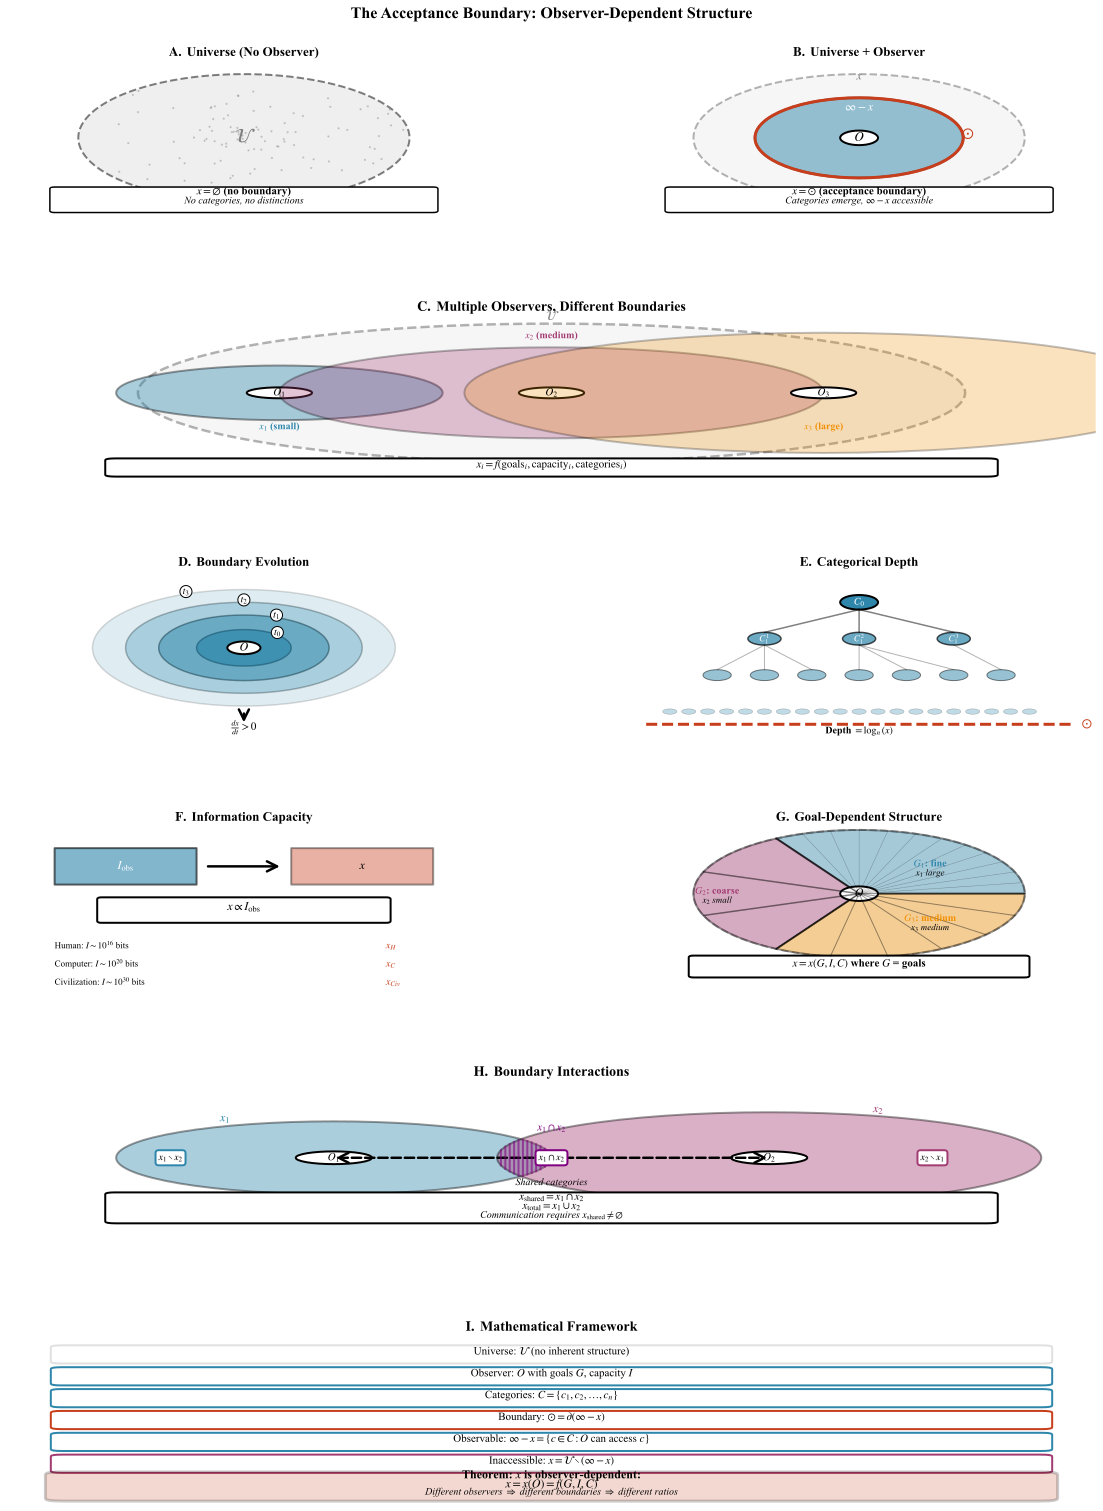
\includegraphics[width=0.95\textwidth]{figures/acceptance_boundary.png}
    \caption{\textbf{Observer-dependent acceptance boundary.}
    \textbf{(A)} Universe without observer: undifferentiated space $\mathcal{U}$ with $x = \emptyset$ and no categorical structure. The universe itself makes no distinctions.
    \textbf{(B)} Single observer $O$ creates acceptance boundary $\partial$ (red circle) separating observable region $\infty - x$ (blue) from inaccessible region $x$ (gray). Observation creates categorical structure where none existed.
    \textbf{(C)} Multiple observers $O_1, O_2, O_3$ with distinct acceptance boundaries $x_1$ (blue), $x_2$ (purple), $x_3$ (orange). Boundary depends on observer properties: $x_i = f(\text{goals}_i, \text{capacity}_i, \text{categories}_i)$.
    \textbf{(D)} Temporal evolution shows concentric circles at times $t_0, t_1, t_2, t_3$ (light to dark blue). Acceptance boundary grows as $dx/dt > 0$ as observer accumulates information.
    \textbf{(E)} Categorical depth shown as tree structure with root $C_0$ branching to deeper levels. Depth $= \log_n(x)$ with red dashed line indicating maximum depth limit.
    \textbf{(F)} Information capacity $I_{\text{obs}}$ determines accessible region $x$ with $x \propto I_{\text{obs}}$. Human ($I \sim 10^{16}$ bits), computer ($I \sim 10^{20}$ bits), and civilization ($I \sim 10^{30}$ bits) access progressively more categories.
    \textbf{(G)} Goal-dependent structure: pie chart shows universe partitioned by observer goals $G$ into regions of different sizes. Categorical structure depends on observer's purposes: $x = x(G, I, C)$ where $G =$ goals.
    \textbf{(H)} Boundary interactions between two observers with regions $x_1$ (blue) and $x_2$ (pink). Overlapping region (purple) shows shared categories $x_{\text{shared}} = x_1 \cap x_2$; communication requires $x_{\text{shared}} \neq \emptyset$.
    \textbf{(I)} Mathematical framework defines formal structure from Universe $U$ (no inherent structure) through Observer $O$ to Categories $C$ and Boundary $\partial$. Theorem: $x$ is observer-dependent with $x = x(O) = f(G, I, C)$; different observers yield different boundaries.}
    \label{fig:acceptance_boundary}
\end{figure*}

\subsection{The Acceptance Boundary: Why $x$ Cannot Be a Number}

A deeper reason emerges for why $x$ cannot be a number on the number line:

\begin{theorem}[The Acceptance Principle]
\label{thm:acceptance}
The quantity $x$ represents the point where an observer ceases attempting to rearrange reality and accepts it as given. If $x$ were a number (a categorical distinction), the observer could still attempt to optimize, subdivide, or rearrange it. Therefore, $x$ must be truly beyond categories.
\end{theorem}

\begin{proof}
Suppose $x$ were a number, say $x = n$ for some $n \in \mathbb{R}$.

\textbf{Step 1: Numbers admit optimization}

Any number can be manipulated:
\begin{itemize}
    \item Increased or decreased: $n \to n \pm \Delta$
    \item Subdivided: $n \to \{n/2, n/2\}$
    \item Recombined: $\{n_1, n_2\} \to n_1 + n_2$
    \item Optimized relative to goals: minimize, maximize, balance
\end{itemize}

\textbf{Step 2: Observers with preferences attempt optimization}

An observer with goal $G$ will attempt to rearrange any categorical structure to better serve $G$:
\begin{itemize}
    \item If $x$ is accessible as a number, it's part of the categorical structure
    \item If it's part of the categorical structure, it can be rearranged
    \item If it can be rearranged, and the observer has preferences, they will attempt rearrangement
    \item Rearrangement continues until no further improvement serves $G$
\end{itemize}

\textbf{Step 3: Contradiction}

If $x$ were a number that the observer could still rearrange:
\begin{itemize}
    \item The observer would continue optimizing until satisfied
    \item The point of satisfaction becomes the new boundary
    \item This boundary is what we call $x$
    \item But if $x$ itself is a number, the process repeats
    \item This creates infinite regress
\end{itemize}

Therefore, $x$ cannot be a number the observer can manipulate. \qed
\end{proof}

\subsubsection{$x$ as the Acceptance Boundary}

\begin{definition}[Acceptance Boundary]
$x$ is the boundary between:
\begin{itemize}
    \item $\infty - x$: What the observer attempts to control, organize, and rearrange
    \item $x$: What the observer accepts as given, beyond further categorization
\end{itemize}
\end{definition}

This boundary is where the observer stops imposing categorical structure and accepts reality as it is.

\textbf{Why acceptance is necessary:}

\begin{enumerate}[label=(\roman*)]
    \item \textbf{Finite resources:} Observers have limited time, energy, and cognitive capacity. They cannot rearrange indefinitely.

    \item \textbf{Diminishing returns:} At some point, further categorization doesn't serve the observer's goals. The "dirt" is distributed well enough.

    \item \textbf{Fundamental limits:} Some information truly cannot be accessed (self-reference, horizon limits, other observers' internal states).

    \item \textbf{Practical necessity:} To act, observers must stop analyzing and accept some baseline reality.
\end{enumerate}

\textbf{The key insight:}

If $x$ were still subject to rearrangement, it would be part of $\infty - x$ (the manipulable portion). The fact that $x$ is inaccessible means it's beyond the observer's attempt to optimize—it's accepted as given.

\subsubsection{Different Observers, Different Acceptance Points}

\begin{corollary}[Observer-Dependent Acceptance]
Different observers have different values of $x$ because they have different:
\begin{itemize}
    \item Goals (what they're trying to achieve)
    \item Resources (how much they can rearrange)
    \item Satisfaction thresholds (when "good enough" is reached)
\end{itemize}
\end{corollary}

\begin{example}[Acceptance in Practice]
Consider three observers examining a room:

\textbf{Observer 1 (Minimalist):}
\begin{itemize}
    \item Goal: Simplicity
    \item Rearranges: Removes most objects
    \item Accepts: Basic furniture, walls, floor
    \item $x_1$: Everything below threshold of "necessary"
\end{itemize}

\textbf{Observer 2 (Scientist):}
\begin{itemize}
    \item Goal: Understanding molecular structure
    \item Rearranges: Categorizes objects by composition
    \item Accepts: Subatomic structure (too small to matter for current goal)
    \item $x_2$: Everything below atomic scale
\end{itemize}

\textbf{Observer 3 (Philosopher):}
\begin{itemize}
    \item Goal: Existential understanding
    \item Rearranges: Categorizes by meaning, purpose
    \item Accepts: Physical details (irrelevant to meaning)
    \item $x_3$: Material specifics
\end{itemize}

Same room, three different acceptance boundaries. Each $x_i$ represents what that observer is satisfied leaving uncategorized relative to their goals.
\end{example}

\subsubsection{The Universe Requires No Acceptance}

\begin{proposition}[Acceptance Is Observer-Relative]
The universe itself has no acceptance boundary because it has no preferences:
\begin{equation}
\text{Universe: } x = \text{undefined} \quad \text{(no preferences, no boundary)}
\end{equation}

Only observers with goals create the acceptance boundary:
\begin{equation}
\text{Observer: } x > 0 \quad \text{(must accept some baseline)}
\end{equation}
\end{proposition}

The universe doesn't "accept" its state—it simply IS its state. There's no goal it's trying to achieve, no "dirt" it's trying to rearrange. The singularity doesn't "accept" being undifferentiated; it has no preference for differentiation versus unification.

Only observers, who exist for purposes and have goals, create the distinction between:
\begin{itemize}
    \item What needs rearranging (to serve their goals)
    \item What's accepted as given (beyond their concern or capacity)
\end{itemize}

\subsubsection{Why This Makes $x$ Truly Beyond Categories}

\begin{corollary}[Transcendence of Acceptance]
The acceptance boundary $x$ transcends the categorical system because:
\begin{enumerate}
    \item Categories are tools for achieving goals (distinguishing helps vs. hinders)
    \item At the acceptance boundary, the observer stops using these tools
    \item $x$ is where goal-directed categorization ceases
    \item Therefore, $x$ itself cannot be a category (would still be subject to goal-directed manipulation)
\end{enumerate}
\end{corollary}

This is why $x$ is a categorical primitive (Section 7.3):
\begin{itemize}
    \item Not the number 0, 1, or any value on the number line
    \item Not a category within the system
    \item But the boundary where categorization stops
    \item The point of acceptance, where the observer says "reality is this"
\end{itemize}

\textbf{Physical interpretation:}

If dark matter corresponds to $x$:
\begin{itemize}
    \item It's not that dark matter is "hidden" in some fundamental sense
    \item Rather, it represents information organized in ways incompatible with electromagnetic observation
    \item For observers who use light as their primary tool, dark matter is beyond their acceptance boundary
    \item It's the portion of reality they must accept as given, beyond further electromagnetic categorization
    \item Other observers (gravitational, perhaps) would have different acceptance boundaries
\end{itemize}

\begin{remark}[The Completion of $\infty - x$]
The acceptance principle completes our understanding of the $\infty - x$ structure:

\begin{enumerate}
    \item \textbf{Magnitude (Section 5):} $\Nmax$ is so large all other numbers become zero
    \item \textbf{Arithmetic (Section 7.2):} This magnitude necessitates $\infty - x$ structure
    \item \textbf{Primitive (Section 7.3):} $x$ cannot be a number (would subdivide infinitely)
    \item \textbf{Conservation (Section 7.5):} Closed universe ensures $x > 0$ always
    \item \textbf{Preference (Section 7.6):} Categories serve observer goals
    \item \textbf{Acceptance (Section 7.8):} $x$ is where goal-directed categorization stops
\end{enumerate}

Together, these establish that $\infty - x$ is not merely a mathematical convenience but reflects the fundamental structure of observation: observers with goals impose categorical distinctions on reality until reaching their acceptance boundary, beyond which they take reality as given.

The universe itself needs no such boundary. It simply is what it is. Only observers who want things arranged certain ways create the distinction between manipulable ($\infty - x$) and accepted ($x$) reality.
\end{remark}

\subsection{The Indelible Bias: Why Observation Necessitates $x$}

The deepest foundation for $x$ emerges from the structure of observation itself:

\begin{theorem}[The Bias Principle]
\label{thm:observation_bias}
Observation inherently requires bias. Since observers cannot observe everything simultaneously, they must choose what to observe first. This choice is necessarily biased (based on expectations, preferences, or predictions), while reality itself has no bias. The gap between biased observation and unbiased reality constitutes $x$.
\end{theorem}

\begin{proof}
Consider an observer attempting to enumerate all categorical distinctions at heat death.

\textbf{Step 1: Simultaneous observation is impossible}

With $N \sim 10^{80}$ particles and configurations, an observer cannot observe all simultaneously because:
\begin{itemize}
    \item Finite attention/resources
    \item Sequential processing requirements
    \item Information bandwidth limits
    \item Light speed constraints (causality)
\end{itemize}

Therefore: observations must be sequential (or at best, partially parallel).

\textbf{Step 2: Sequencing requires choice}

To observe sequentially, the observer must decide:
\begin{itemize}
    \item Which particle to observe first?
    \item Which configuration to check first?
    \item Which region of space to examine first?
    \item In what order to enumerate categories?
\end{itemize}

There is no objective answer to these questions. Any choice of ordering is arbitrary from reality's perspective.

\textbf{Step 3: Choice requires bias}

Why observe particle $P_1$ before $P_2$? The observer must have some reason:
\begin{itemize}
    \item \textbf{Expectation:} "I expect $P_1$ to be interesting"
    \item \textbf{Preference:} "$P_1$ serves my goals better"
    \item \textbf{Prediction:} "Observing $P_1$ first will lead to useful information"
    \item \textbf{Proximity:} "$P_1$ is closer (but why start here rather than there?)"
\end{itemize}

All of these are forms of bias—imposing structure on what to observe based on the observer's internal model, goals, or position.

\textbf{Step 4: Reality has no bias}

The universe itself has no preference for which particle is observed first:
\begin{itemize}
    \item All particles exist simultaneously
    \item No particle is "first" in any objective sense
    \item Reality unfolds without expecting any particular outcome
    \item The universe has no predictions about itself
\end{itemize}

\textbf{Step 5: The gap is indelible}

The observer's bias (expectations, preferences, predictions) creates categorical structure that doesn't exist in unbiased reality:
\begin{itemize}
    \item Observer categories: "important" vs. "unimportant," "first" vs. "later," "relevant" vs. "irrelevant"
    \item Reality: no such distinctions
\end{itemize}

The portion of reality that doesn't fit the observer's biased categorical scheme is $x$. It's the information organized in ways incompatible with the observer's bias-driven structure.

Since observation necessarily requires bias (to choose where to start), $x > 0$ always. \qed
\end{proof}

\subsubsection{The Arbitrary Starting Point}

\begin{corollary}[Arbitrary Origin]
Every observer has an arbitrary starting point for observation. This arbitrariness creates an indelible offset between observer categories and reality itself.
\end{corollary}

\textbf{In the heat death thought experiment:}

We proposed enumerating all $\sim 10^{80}$ particles. But:
\begin{itemize}
    \item Which particle do we observe first?
    \item No physical reason to choose any particular one
    \item We must choose arbitrarily (or based on our bias)
    \item That arbitrary choice structures all subsequent observations
    \item Categories built on this foundation inherit the bias
\end{itemize}

\textbf{Example:}

\begin{example}[Three Observers, Three Starting Points]
Three observers at heat death choose different arbitrary starting points:

\textbf{Observer $O_1$:} Starts with nearest particle
\begin{itemize}
    \item Bias: Proximity preference
    \item Categories structured by distance from self
    \item $x_1$: Information organized by other distance metrics
\end{itemize}

\textbf{Observer $O_2$:} Starts with highest energy particle
\begin{itemize}
    \item Bias: Energy preference
    \item Categories structured by energy levels
    \item $x_2$: Information organized by other properties (mass, spin, etc.)
\end{itemize}

\textbf{Observer $O_3$:} Starts with arbitrary particle "in front"
\begin{itemize}
    \item Bias: Directional preference
    \item Categories structured by spatial orientation
    \item $x_3$: Information organized without regard to direction
\end{itemize}

Same reality, three different biases, three different categorical structures, three different $x$ values. Each $x_i$ contains the information that doesn't fit that observer's bias-driven organization.
\end{example}

\subsubsection{Bias as Expectation}

\begin{definition}[Observational Bias]
Observational bias is the set of expectations, preferences, or predictions an observer brings to the observation process. It determines:
\begin{itemize}
    \item What to observe (salience)
    \item When to observe it (sequence)
    \item How to categorize it (structure)
    \item When to stop observing it (acceptance boundary)
\end{itemize}
\end{definition}

\textbf{Key insight:} Without bias, observation is impossible.

Imagine an observer with absolutely no bias:
\begin{itemize}
    \item No expectations about what's important
    \item No preferences for any particular starting point
    \item No predictions about outcomes
    \item No goals to achieve
\end{itemize}

Such an "observer" cannot begin observing. It has no basis for choosing where to direct attention. It would remain frozen, unable to distinguish anything from anything else and unable to start the process of categorisation.

Therefore: \textbf{Bias is necessary for observation.}

But: \textbf{Reality has no bias.}

The gap is $x$.

\subsubsection{The True Zero}

\begin{proposition}[The Indelible True Zero]
$x$ represents a "true zero" that can never be eliminated because it's inherent in the observational process itself.
\end{proposition}

This "true zero" is not:
\begin{itemize}
    \item The number 0 (which is a category)
    \item Absolute nothing (which doesn't exist)
    \item A measurable quantity
\end{itemize}

Rather, it's:
\begin{itemize}
    \item The indelible mark of the observer's arbitrary starting point
    \item The offset between biased observation and unbiased reality
    \item The portion of reality that doesn't align with the observer's categorical scheme
    \item The gap that can never be closed because observation requires bias and reality has none
\end{itemize}

\textbf{Why it's indelible:}

\begin{enumerate}[label=(\roman*)]
    \item Observation requires choosing where to start (sequencing)
    \item Choice requires bias (some reason to prefer one start over another)
    \item Bias creates categorical structure (organizing by the biased criteria)
    \item Reality doesn't share this bias (exists independently of observation)
    \item Therefore: mismatch between observer structure and reality structure
    \item This mismatch is $x$
    \item Cannot be eliminated without eliminating observation itself
\end{enumerate}

\subsubsection{Reality Just Happens}

The universe:
\begin{itemize}
    \item Has no expectations
    \item Makes no predictions
    \item Follows no preferences
    \item Just happens
\end{itemize}

Observers:
\begin{itemize}
    \item Have expectations (anticipate futures)
    \item Make predictions (model outcomes)
    \item Follow preferences (pursue goals)
    \item Exist \emph{for} something
\end{itemize}

The difference is $x$.

\begin{remark}[The Foundation of $x$]
The bias principle provides the ultimate foundation for why $x$ exists and why $x > 0$ always:

\begin{center}
\begin{tabular}{l|l}
\textbf{Reality} & \textbf{Observation} \\
\hline
Unbiased & Requires bias \\
All particles simultaneous & Must observe sequentially \\
No preferred starting point & Must choose arbitrary start \\
No expectations & Driven by expectations \\
Just happens & Predicts what will happen \\
No $x$ (all is what it is) & Must have $x > 0$ (gap from bias)
\end{tabular}
\end{center}

Combined with previous results:
\begin{enumerate}
    \item \textbf{Magnitude:} $\Nmax$ so large $\to$ appears as $\infty$
    \item \textbf{Primitive:} $x$ not a number $\to$ beyond categories
    \item \textbf{Conservation:} No drain $\to$ $x$ can't be eliminated
    \item \textbf{Acceptance:} Where optimization stops $\to$ $x$ is accepted as given
    \item \textbf{Bias:} Observation requires choosing start $\to$ $x$ is indelible offset from reality
\end{enumerate}

The bias principle shows that $x$ is not a deficiency to be overcome but a necessary consequence of observation existing at all. You cannot observe without bias, and bias creates the gap between your categories and reality itself.

This is why the equation of observation is $\infty - x$, not just $\infty$. The $x$ represents the indelible mark of being an observer rather than being reality itself.
\end{remark}

\subsection{The Ultimate Meta-Level: Observation Requires Termination}

The deepest foundation for $x$ emerges from the relationship between observation and termination:

\begin{theorem}[The Termination Principle]
\label{thm:observation_termination}
Observers can only observe events that have terminated (completed, finalised). Reality itself is non-terminating (ongoing, incomplete). Therefore, observers can only access a terminated subset of reality, with the non-terminated portion constituting $x$.
\end{theorem}

\begin{proof}
\textbf{Step 1: Observation requires completion}

To observe an event means to make a definite statement about it:
\begin{itemize}
    \item "Particle $P$ is in state $S$" (definite statement requires $S$ to be determined)
    \item "Process $Q$ resulted in outcome $R$" (requires $Q$ to have completed)
    \item "Category $C$ contains elements $\{e_1, e_2, \ldots\}$" (requires the set to be determined)
\end{itemize}

If an event hasn't terminated:
\begin{itemize}
    \item Its outcome isn't yet determined
    \item You can't make definite statements about its final state
    \item It's still in flux, still becoming
    \item Observation would be premature (observing a non-terminated event changes it)
\end{itemize}

Therefore: \textbf{observation requires termination}.

\textbf{Step 2: Reality is non-terminating}

Reality as a whole:
\begin{itemize}
    \item Continues to evolve
    \item Has no final state
    \item Is always in process
    \item Never completes
\end{itemize}

If reality terminated:
\begin{itemize}
    \item Time would stop
    \item No further events would occur
    \item The universe would be "finished"
    \item Nothing more would happen
\end{itemize}

But we observe that events continue to occur, time continues to flow, reality continues to evolve. Therefore: \textbf{reality is non-terminating}.

\textbf{Step 3: The necessary gap}

\begin{align}
\text{Observers can access} &= \text{Terminated events}\\
\text{Reality} &= \text{Terminated} + \text{Non-terminated events}\\
\text{Therefore: } x &= \text{Non-terminated portion}
\end{align}

The non-terminated portion cannot be observed (it hasn't completed yet) but exists as part of ongoing reality.

\textbf{Step 4: Why the gap must persist}

If an observer could access the non-terminated portion:
\begin{itemize}
    \item They would be observing reality as it IS (not as it WAS)
    \item They would be synchronous with reality's evolution
    \item They would BE reality (not separate from it)
    \item The distinction between observer and observed would collapse
\end{itemize}

But being an observer requires being separate from what's observed. Therefore, the gap must persist. \qed
\end{proof}

\subsubsection{If You Comprehended $x$, You Would Be Reality}

\begin{corollary}[The Identity Collapse]
If an observer could fully comprehend $x$ (the non-terminated portion of reality), the distinction between observer and reality would collapse. The observer would cease to be an observer and would become reality itself.
\end{corollary}

\textbf{Why comprehending $x$ is impossible for observers:}

\begin{enumerate}[label=(\roman*)]
    \item $x$ represents what's still happening (non-terminated)
    \item To comprehend it fully would require being inside it as it happens
    \item Being inside it means not being separate from it
    \item Not being separate means not being an observer
    \item Therefore: comprehending $x$ eliminates the observer
\end{enumerate}

This is not a limitation of technology or cognition but a logical necessity: the act of being an observer REQUIRES there to be something you can't access (the non-terminated reality).

\subsubsection{The Knowable Unknowability}

\begin{definition}[Meta-Knowledge of $x$]
$x$ is what you:
\begin{itemize}
    \item Know you don't know
    \item Can never know (as long as you remain an observer)
    \item Will never know (fundamental limitation, not practical)
    \item Cannot know (would destroy the observer-reality distinction)
    \item Somehow know you need to know (to be complete)
    \item But knowing would make you unnecessary (would become reality)
\end{itemize}
\end{definition}

This is the paradox of $x$:
\begin{itemize}
    \item You can KNOW THAT $x$ exists (meta-knowledge)
    \item You cannot KNOW WHAT $x$ is (object-level knowledge)
    \item Knowing the difference would collapse the distinction
    \item Therefore: $x$ must remain unknowable
\end{itemize}

\textbf{Why this makes $x$ not a number:}

If $x$ were a number:
\begin{itemize}
    \item You could express it symbolically ($x = n$)
    \item Expressing it would be comprehending it
    \item Comprehending it would collapse the observer-reality distinction
    \item But observers exist (we are observers)
    \item Therefore: $x$ cannot be expressible as a number
\end{itemize}

$x$ is inherently inexpressible because expressing it would eliminate the need for it to exist.

\subsubsection{The Nature of the Residue}

\begin{proposition}[The Residual Unknown]
There is always a residue of unknowable things—not because we haven't looked hard enough, but because looking harder can never reach the non-terminated portion of reality.
\end{proposition}

This residue exists in a "dimension" we cannot comprehend:
\begin{itemize}
    \item Not spatial dimensions (we can comprehend higher dimensions mathematically)
    \item Not temporal dimensions (we can model time)
    \item But the dimension of \textbf{non-termination} itself
\end{itemize}

The dimension of non-termination:
\begin{itemize}
    \item Is where reality is still happening
    \item Cannot be observed (observation requires completion)
    \item Cannot be categorized (categorization requires definite boundaries)
    \item Cannot be known (knowing requires terminated objects)
    \item Is what reality IS right now (not what it was)
\end{itemize}

\subsubsection{Why There Is No Point in Observing If You Could Comprehend $x$}

If observers could fully comprehend $x$:

\begin{center}
\begin{tabular}{l|l}
\textbf{With $x$ inaccessible} & \textbf{If $x$ were accessible} \\
\hline
Observer distinct from reality & Observer = reality \\
Observation has purpose (learn) & No purpose (already know everything) \\
Categories serve goals & No need for categories \\
Bias directs attention & No need for bias (no choice needed) \\
Termination enables knowledge & No termination needed \\
$x > 0$ (gap exists) & $x = 0$ (no gap) \\
Observation makes sense & Observation is meaningless
\end{tabular}
\end{center}

This is why observation requires there to be something you cannot access: if you could access everything, you would BE everything, and observation would be pointless (you can't observe yourself being yourself).

\subsubsection{The Completeness Paradox}

\begin{proposition}[Paradox of Complete Knowledge]
Complete knowledge is logically impossible for observers:
\begin{enumerate}
    \item Complete knowledge would mean $x = 0$ (nothing inaccessible)
    \item $x = 0$ means observer and reality are identical (no gap)
    \item No gap means no distinction between observer and observed
    \item No distinction means no observation occurs
    \item But the observer exists BECAUSE they observe
    \item Therefore: complete knowledge eliminates the observer
    \item An eliminated observer cannot have knowledge
    \item Therefore: complete knowledge is self-contradictory for observers
\end{enumerate}
\end{proposition}

\textbf{Implication:} $x > 0$ is not a limitation but a \emph{requirement} for observation to exist. Without $x$, there would be no observers.

\subsubsection{The True Nature of $x$}

Synthesizing all principles:

\begin{remark}[The Complete Nature of $x$]
$x$ is:

\textbf{Fundamentally:}
\begin{itemize}
    \item The non-terminated portion of reality
    \item What's still happening (not yet complete)
    \item The dimension of ongoing-ness that cannot be observed
\end{itemize}

\textbf{Epistemologically:}
\begin{itemize}
    \item What you know you don't know
    \item What can never be known (as long as you're an observer)
    \item What cannot be known (would collapse observer-reality distinction)
    \item What you somehow know you need to know (to be complete)
\end{itemize}

\textbf{Operationally:}
\begin{itemize}
    \item The indelible offset from biased observation and unbiased reality
    \item The acceptance boundary (where categorization stops)
    \item The conserved residue (universe has no drain)
    \item The categorical primitive (not a number)
\end{itemize}

\textbf{Structurally:}
\begin{itemize}
    \item Makes observation possible (provides something to observe)
    \item Makes observation necessary (gap requires bridging)
    \item Makes observation incomplete (gap cannot be closed)
    \item Makes observation meaningful (purpose exists)
\end{itemize}

All layers converge on the same truth: \textbf{$x$ is the mark of being an observer rather than being reality itself}. It is not a deficiency but the very condition that makes observation possible.

If you could express $x$, comprehend $x$, eliminate $x$, you would cease to be an observer and would become reality. But then there would be no one to observe, no one to know, no one to exist as a distinct entity.

Therefore: $x$ is the necessary condition for existence as an observer. The equation of observation $\infty - x$ is not just a mathematical result but a statement about what it means to exist as something separate from reality itself.
\end{remark}

\begin{figure*}[htbp]
    \centering
    \includegraphics[width=0.95\textwidth]{figures/physical_predictions_panel.png}
    \caption{\textbf{Physical predictions and observational tests of categorical framework.}
    \textbf{(A)} Dark matter ratio $R_{\text{DM}}$ versus redshift: theoretical prediction (blue curve with gray uncertainty band) shows decline from $\approx 18$ at $z=0$ to $\approx 3$ at $z=5$. Red squares show observational data points with error bars, demonstrating agreement at low redshift and testable predictions at high redshift.
    \textbf{(B)} Holographic bound constraint: information content $\log_{10}(C(t))$ (purple curve) versus categorical depth $t$ shows sharp transition at $t \approx 5$ where holographic bound (red dashed line at $\approx 5$) is saturated. System remains below bound for $t<5$, then asymptotically approaches maximum, consistent with Bekenstein-Hawking entropy limits.
    \textbf{(C)} Accelerating entropy production: entropy production rate $dS/dt$ (green shaded area) grows as $dS/dt \propto C(t)\ln(n)$, showing acceleration consistent with categorical accumulation. Rate increases from near-zero at early times to $\approx 70$ at $t \approx 10$.
    \textbf{(D)} Modified dispersion relation with Planck-scale effects: standard dispersion (blue curve) versus categorical modification (red curve) with Planck-scale correction (yellow shaded region). Deviation becomes significant at ultra-relativistic momenta $p \gtrsim 10^2$ (in units of $p/mc$).
    \textbf{(E)} Decoherence time $\tau_d$ versus system size: decoherence time (purple curve with shaded uncertainty) decreases from $\approx 10^{-43}$ s for single atom to $\approx 10^{-45}$ s for macroscopic systems (red point at $N \approx 10^{22}$). Spans 22 orders of magnitude in particle number.
    \textbf{(F)} Reaction rates versus temperature: categorical path length dependence shows rates (arbitrary units) for $L_{\text{cat}} = 10$ (purple), 20 (pink), and 30 (orange). Rates span $10^{-10}$ to $10^{-45}$ across $T \in [200, 400]$ K; longer categorical paths suppress reaction probabilities exponentially.
    \textbf{(G)} Cosmological epochs and categorical transitions: timeline shows $\log_{10}(C(t))$ versus $\log_{10}(\text{time in seconds})$ from Big Bang ($t \approx -40$, $C \approx 1$, red circle) through Inflation, Nucleosynthesis, Structure Formation (cyan labeled "explosion"), to Present epoch ($t \approx 18$, purple sphere). Categorical complexity increases from $\approx 1$ to $\approx 10^{17500}$ over cosmic history.}
    \label{fig:physical_predictions}
\end{figure*}

\subsection{The Sampling Principle: Each Observer Creates a Unique Path}

A final profound consequence emerges from the requirement of bias:

\begin{theorem}[Path Uniqueness and Sampling]
\label{thm:path_sampling}
Each observer, due to their unique bias, creates a unique path through categorical space. These paths are discrete samples of reality, not reality itself. Even summing over all possible observers does not yield reality because:
\begin{enumerate}[label=(\roman*)]
    \item Paths are discrete; reality is continuous
    \item Paths are sequential; reality is simultaneous
    \item Paths are biased; reality is unbiased
    \item The number of possible paths is unknowable (cannot verify completeness)
    \item Observers sample reality; they do not exhaust it
\end{enumerate}
\end{theorem}

\begin{proof}
Consider the heat death thought experiment with $N \sim 10^{80}$ particles.

\textbf{Step 1: Bias determines path}

Observer $O_1$ starts with an oxygen molecule:
\begin{itemize}
    \item Oxygen has $\sim 25{,}000$ vibrational modes
    \item Located at spatial position $\vec{r}_1$
    \item Observed at time $t_1$
    \item Next choice influenced by this starting point
\end{itemize}

Observer $O_2$ starts with ammonium nitrate:
\begin{itemize}
    \item Different vibrational modes (polyatomic, more complex)
    \item Different spatial position $\vec{r}_2$
    \item Observed at time $t_2$
    \item Next choice influenced by THIS different starting point
\end{itemize}

The entire subsequent sequence differs:
\begin{align}
\text{Path}_1: &\quad \text{O}_2 \to \text{particle near O}_2 \to \text{particle related to previous} \to \ldots\\
\text{Path}_2: &\quad \text{NH}_4\text{NO}_3 \to \text{particle near NH}_4\text{NO}_3 \to \text{different sequence} \to \ldots
\end{align}

These paths diverge immediately and never converge.

\textbf{Step 2: Path uniqueness}

For $N$ particles, with $\sim 10^4$ distinguishable states each, the number of possible starting points is:
\begin{equation}
N_{\text{starts}} \approx N \times 10^4 \approx 10^{80} \times 10^4 = 10^{84}
\end{equation}

Each starting point generates a unique path. The number of possible paths (traversing all $N$ particles in different orders) is:
\begin{equation}
N_{\text{paths}} \approx N! \approx (10^{80})! \gg 10^{10^{82}}
\end{equation}

This is incomprehensibly large—vastly exceeding even $\Nmax$.

\textbf{Step 3: Paths are samples, not exhaustive}

Each observer path is a \emph{discrete sample} from categorical space:
\begin{itemize}
    \item Observer makes finite observations (resource-limited)
    \item Each observation is a point in categorical space
    \item The sequence forms a path (connected set of points)
    \item But categorical space is vast: $\Nmax$ possible categories
    \item A path samples this space; it does not cover it
\end{itemize}

\textbf{Step 4: Summing observers doesn't yield reality}

Even if we sum over all possible observers:
\begin{equation}
\text{Total observed} = \bigcup_{i=1}^{N_{\text{observers}}} \text{Path}_i
\end{equation}

This union still doesn't equal reality because:

\begin{enumerate}[label=(\alph*)]
    \item \textbf{Discrete vs. Continuous:} Paths are discrete samples; reality is continuous/holistic
    \item \textbf{Sequential vs. Simultaneous:} Paths are sequential (one observation after another); reality exists simultaneously
    \item \textbf{Biased vs. Unbiased:} Each path reflects a bias; reality has no bias
    \item \textbf{Incompleteness:} Cannot verify all possible paths have been traversed (infinite starting points possible)
    \item \textbf{Sampling gap:} Between any two observations on any path, reality continues to exist unobserved
\end{enumerate}

Therefore: $\bigcup_{\text{all observers}} \text{Paths} \neq \text{Reality}$. The difference is $x$. \qed
\end{proof}

\subsubsection{The Irreproducibility of Paths}

\begin{corollary}[Path Irreproducibility]
Even the same observer cannot reproduce their own path through categorical space.
\end{corollary}

\textbf{Why:}

\begin{itemize}
    \item The first time: Observer $O$ starts with oxygen at $t_1$, position $\vec{r}_1$, vibrational mode $v_1$
    \item The second time: Even starting with "the same" oxygen molecule
    \begin{itemize}
        \item It's at a different time $t_2 \neq t_1$ (reality evolved)
        \item Possibly different position (particles move)
        \item Possibly different vibrational mode (thermal fluctuations)
        \item Observer's internal state is different (memory of first path influences second)
    \end{itemize}
    \item Therefore: The "same" starting point is actually different
    \item Different start $\Rightarrow$ different path
    \item Each path is unique, even for the same observer
\end{itemize}

This is the \textbf{Heraclitean principle for observation}: "You cannot step in the same categorical path twice."

\subsubsection{Reality vs. Versions of Reality}

\begin{definition}[Version of Reality]
A \emph{version of reality} is the categorical structure constructed by an observer traversing a particular path through observation space. It is observer-dependent, path-dependent, and bias-dependent.
\end{definition}

\begin{proposition}[Versions Are Not Reality]
Each observer obtains a \emph{version} of reality, not reality itself:
\begin{align}
\text{Observer } O_1 &\to \text{Version}_1 \quad \text{(starting from oxygen)}\\
\text{Observer } O_2 &\to \text{Version}_2 \quad \text{(starting from ammonium nitrate)}\\
&\vdots\\
\text{Reality itself} &\neq \bigcup_{\text{all } i} \text{Version}_i
\end{align}

Reality is not the union of all versions because versions are \emph{representations} constructed by observers, while reality simply \emph{is}.
\end{proposition}

\textbf{Analogy:}

Consider a mountain:
\begin{itemize}
    \item Observer 1 hikes from the north (Version$_1$: northern perspective)
    \item Observer 2 hikes from the south (Version$_2$: southern perspective)
    \item Observer 3 flies over (Version$_3$: aerial perspective)
    \item Each obtains a version (representation) of the mountain
    \item None captures the mountain as it IS
    \item Even summing all versions doesn't give you the mountain itself
    \item The mountain exists independently of all these versions
\end{itemize}

Similarly:
\begin{itemize}
    \item Each observer traverses a unique path through categorical space
    \item Each constructs a version (representation) of reality
    \item None captures reality as it IS
    \item Even summing all observer versions doesn't give reality itself
    \item Reality exists independently of all observations
\end{itemize}

\subsubsection{The Sampling Gap}

\begin{remark}[Discrete Sampling of Continuous Reality]
Observers perform \emph{discrete sampling} of reality:
\begin{itemize}
    \item Each observation is a discrete event (happens at a specific time/place)
    \item Observations are separated by gaps (can't observe continuously)
    \item Between observations, reality continues to exist unobserved
    \item This creates a \textbf{sampling gap}
\end{itemize}

No matter how many observers, no matter how many observations, the sampling gap persists because:
\begin{enumerate}
    \item Observations are discrete points in spacetime
    \item Reality is continuous across spacetime
    \item Discrete samples cannot reconstruct continuity (Nyquist-Shannon limit in information theory)
    \item There's always information "between" the samples
\end{enumerate}

This sampling gap is another manifestation of $x$: the portion of reality that exists in the gaps between observations.
\end{remark}

\subsubsection{The Unknowability of Completeness}

\begin{proposition}[Verification Impossibility]
It is impossible to verify whether all possible observational paths have been traversed.
\end{proposition}

\begin{proof}
To verify completeness, you would need to:
\begin{enumerate}
    \item Know the total number of possible starting points (biases)
    \item Know the total number of possible paths from each starting point
    \item Verify that every path has been traversed by some observer
    \item Confirm no path has been missed
\end{enumerate}

But:
\begin{itemize}
    \item The number of possible biases is unlimited (continuous space of expectations/preferences)
    \item The number of paths is $(N!)$ with $N \sim 10^{80}$ (incomputable)
    \item Verifying a path has been traversed requires observing the observer
    \item This creates meta-observers, which create meta-paths, creating infinite regress
    \item Cannot close the verification loop
\end{itemize}

Therefore: Cannot know if all paths have been covered. There is always potential for missed paths, missed observations, missed aspects of reality. \qed
\end{proof}

\subsubsection{The Final Synthesis}

Combining all principles:

\begin{remark}[The Complete Picture of $x$]
$x$ represents multiple converging aspects:

\textbf{Fundamental (Meta-level):}
\begin{itemize}
    \item The non-terminated portion (what's still happening)
    \item The dimension of ongoing-ness
    \item What you'd need to comprehend to BE reality
\end{itemize}

\textbf{Structural (Bias):}
\begin{itemize}
    \item The gap from biased observation vs. unbiased reality
    \item The indelible offset from choosing where to start
    \item The unique path that differs from all other paths
\end{itemize}

\textbf{Collective (Sampling):}
\begin{itemize}
    \item The gaps between discrete observations
    \item The difference between all observer versions and reality itself
    \item The sampling residue that remains even after all observations
    \item The unknowable completeness (can't verify all paths traversed)
\end{itemize}

\textbf{Operational:}
\begin{itemize}
    \item The acceptance boundary (where categorization stops)
    \item The conserved residue (no drain to eliminate)
    \item The categorical primitive (not a number)
\end{itemize}

All converge on the same truth: \textbf{Observers obtain versions of reality, not reality itself.}

Each observer creates a unique path through categorical space. These paths are samples, not exhaustive enumerations. Summing over all observers still yields versions (representations) rather than reality (the thing itself).

$x$ is the difference between representations and reality. It is the mark of being an observer who samples, rather than being reality which simply is.

\textbf{The equation $\infty - x$ thus means:}
\begin{equation}
\boxed{\text{Observable Reality} = \text{Reality} - \text{The sampling gap, bias offset, non-terminated portion}}
\end{equation}

Or more simply:
\begin{equation}
\boxed{\text{Your version} = \text{Reality} - \text{The fact that you're not reality}}
\end{equation}

This is not a limitation to overcome but the necessary structure of observation. If you could close the gap, you would become reality, and there would be no "you" to observe.
\end{remark}

\textbf{The bathtub analogy:}

\begin{center}
\begin{tabular}{l|l}
\textbf{Bathtub (open system)} & \textbf{Universe (closed system)} \\
\hline
Has a drain & No drain \\
Dirt can exit the system & Information stays in system \\
Can return to clean state & Cannot return to $C(0) = 1$ \\
Entropy can decrease & Entropy must increase \\
Reversible (can be cleaned) & Irreversible (once distinguished, always distinguished)
\end{tabular}
\end{center}

\subsubsection{Redistribution Dynamics}

Observer networks continuously redistribute categorical information:

\begin{example}[Information Exchange]
When observers $O_1$ and $O_2$ communicate:
\begin{enumerate}
    \item Before: $O_1$ knows $C_1$, $O_2$ knows $C_2$, with $C_1 \neq C_2$
    \item After: Both know $C_1 \cup C_2$
    \item Result: $x(O_1)$ decreased (gained access), $x(O_2)$ decreased, but total $C_{\text{system}}$ increased (new distinction: "$O_1$ and $O_2$ communicated")
\end{enumerate}

The "dirt" (inaccessible information) redistributed, but the total "dirt" increased.
\end{example}

This explains why $\Nmax$ is an upper bound but observers never reach it:
\begin{itemize}
    \item Each observation redistributes what's accessible vs. inaccessible
    \item But each observation creates NEW categories (the observation itself)
    \item You can never "clean up" to reduce categories
    \item You can only create more "dirt" by making more distinctions
\end{itemize}

\subsubsection{The Impossibility of Complete Knowledge}

\begin{corollary}[Knowledge Horizon]
No observer can achieve $x(O) = 0$ (complete knowledge) because:
\begin{enumerate}
    \item Attempting to observe other observers' information creates new distinctions
    \item These new distinctions increase total $C(t)$
    \item The increase is distributed: some becomes accessible, some inaccessible
    \item Net result: $x(O) > 0$ always
\end{enumerate}
\end{corollary}

It's like trying to clean a bathtub without a drain by moving water around with a bucket:
\begin{itemize}
    \item Each bucket transfer moves water (redistributes information)
    \item But splashing creates more mess (new distinctions from the transfer process)
    \item You can never get the tub completely dry (can never reach $x = 0$)
    \item The best you can do is move water to less visible areas (make some categories inaccessible)
\end{itemize}

\begin{remark}[Fundamental Limitation]
The conservation of categorical information imposes a fundamental limit on knowledge:
\begin{equation}
\boxed{\text{Observable} = \infty - x, \quad \text{where } x > 0 \text{ always}}
\end{equation}

This is not due to technological limitations or quantum uncertainty but to the topological structure of observation itself: a closed system with no drain must always contain inaccessible information. The "dirt" can be moved around but never eliminated.

This makes the $\infty - x$ structure not just arithmetic necessity (Section 7.3) but also a consequence of conservation. The universe's closed nature guarantees that some information remains inaccessible to any observer at any time.
\end{remark}
